\section{Experiments}
\begin{figure*}[t]
  \centering
   \includegraphics[width=1\textwidth]{Figures/errormap_dynamic_3.pdf}
   
   \caption{Qualitative comparison of range estimation on \textit{Waymo Dynamic} dataset. Dynamic vehicles are zoomed in, and points are color-coded by range errors~(-100 \bwrDyNFL~100 cm).
   }
   \label{fig:errormap_dynamic}
   
\end{figure*}








\subsection{Datasets and evaluation protocol}\label{sec:datasets}

\paragraph{Real-world Dynamic scenes.} 
We construct \textit{Waymo Dynamic} dataset by selecting four representative scenes from Waymo Open dataset~\cite{sun2020scalability}, with multiple moving vehicles inside. These scenes are comprised of sequences of 50 consecutive frames. For evaluation purposes, every fifth frame is designated for testing, while the other 40 frames are allocated for training.


\paragraph{Real-world static scenes.}
We also evaluate our method on four static scenes as introduced in~\cite{Huang2023nfl}. There are two settings, \textit{Waymo Interp} applies the same evaluation protocol as \textit{Waymo Dynamic}, while \textit{Waymo NVS} employs a dedicated closed-loop evaluation to validate the real novel view synthesis performance. Please refer to NFL~\cite{Huang2023nfl} for more details about this setting. 
 


\paragraph{Synthetic static scenes.}  
\textit{TownClean} and \textit{TownReal} are synthetic static scenes introduced in NFL~\cite{Huang2023nfl}. They consist of 50 LiDAR scans simulated in urban street environment, using non-diverging and diverging beams, respectively. 



\paragraph{Evaluation metrics.}\label{sec:metrics}
To evaluate the LiDAR range accuracy, we employ a suite of four metrics: mean absolute errors~(MAE [cm]), median absolute errors~(MedAE [cm]), Chamfer distance~(CD[cm]) and MedAE for dynamic vehicles~(MedAE Dyn[cm]). For intensity evaluation, We report root mean square error~(RMSE).
%
In addition to our primary evaluations, we assess the re-simulated LiDAR scans' realism through two auxiliary tasks: object detection and semantic segmentation. For object detection, we calculate the \textit{detection agreement}~\cite{manivasagam2020lidarsim}, both for all vehicles (Agg.~[\%]) and specifically for dynamic vehicles (Dyn.$\;$Agg.~[\%]). Regarding semantic segmentation, we measure and report recall, precision, and the intersection over union (IoU[\%]). It's important to note that the predictions on the original LiDAR scans serve as our \textit{ground truth}, against which we compare the results obtained from the re-simulated scans.




\paragraph{Baseline methods.}
Regarding LiDAR simulation on static scenes, NFL~\cite{Huang2023nfl} and LiDARsim\cite{manivasagam2020lidarsim} are two closest baselines to compare to. Additionally, we include i-NGP~\cite{mueller2022instant}, DS-NeRF~\cite{kangle2021dsnerf}, and URF~\cite{rematas2022urban} for comparison. As for simulation on dynamic scenes, we compare to LiDARsim~\cite{manivasagam2020lidarsim} and UniSim~\cite{yang2023unisim}\footnote{We re-implement LiDARsim~\cite{lee2015lidar} and UniSim~\cite{yang2023unisim} as they are not open-sourced.}. Please refer to the supplementary for implementation details.


\begin{table}[t]
    \setlength{\tabcolsep}{4pt}
    \renewcommand{\arraystretch}{1.2}
	\centering
	\resizebox{\columnwidth}{!}{
    \begin{tabular}{l|ccccc}
    \toprule
    Method  & MAE $\downarrow$ &  MedAE $\downarrow$ & CD $\downarrow$ & MedAE Dyn $\downarrow$ & Intensity RMSE $\downarrow$\\
    \midrule
    LiDARsim~\cite{manivasagam2020lidarsim} & 170.1 & 11.5 & 31.1 &  16.0  & 0.10\\
    Unisim~\cite{yang2023unisim} & 35.6 & 6.1 & 14.3 &14.3 & \textbf{0.05}\\
    Ours~ & \textbf{30.8} & \textbf{3.0} & \textbf{10.9} &\textbf{8.5} & \textbf{0.05}\\
    \bottomrule
    \end{tabular}
    }
    
	\caption{Evaluation of LiDAR NVS on \textit{Waymo Dynamic} dataset.}
	\label{tab:waymodynamic}
\end{table}
\begin{table}[t]
    \setlength{\tabcolsep}{4pt}
    \renewcommand{\arraystretch}{1.2}
	\centering
	\resizebox{\columnwidth}{!}{
    \begin{tabular}{l|ccc|ccc|ccc|ccc}
    \toprule
    & \multicolumn{3}{c|}{TownClean}& \multicolumn{3}{c|}{TownReal} & \multicolumn{3}{c|}{Waymo interp.} & \multicolumn{3}{c}{Waymo NVS} \\
    Method  & MAE $\downarrow$ &  MedAE $\downarrow$ & CD $\downarrow$& MAE $\downarrow$ &  MedAE $\downarrow$ & CD $\downarrow$ & MAE $\downarrow$ &  MedAE $\downarrow$ & CD $\downarrow$ & MAE $\downarrow$ &  MedAE $\downarrow$ & CD $\downarrow$\\
    \midrule
    i-NGP~\cite{mueller2022instant} &42.2 &4.1 & 17.4 & 49.8 & 4.8 & 19.9 & \textbf{26.4} & 5.5 & \textbf{11.6} & \underline{30.4} & 7.3 & 15.3\\
    DS-NeRF~\cite{kangle2021dsnerf} &41.7 & 3.9 &16.6 & 48.9 & 4.4 & 18.8 & \underline{28.2} & 6.3 & 14.5 & 30.4 & 7.2 & 16.8 \\
    URF~\cite{rematas2022urban} &43.3&4.2&16.8& 52.1 & 5.1 & 20.7 & 28.2 & 5.4 & 12.9 & 43.1 & 10.0 & 21.2 \\
    LiDARsim~\cite{manivasagam2020lidarsim} &159.6&\underline{0.8}&23.5& 162.8 & 3.8 & 27.4 & 116.3 & 15.2 & 27.6 & 160.2 & 16.2 & 34.7 \\
    NFL\cite{Huang2023nfl}  &\underline{32.0}&2.3&\underline{9.0}& \underline{39.2} & \underline{3.0} & \underline{11.5} & 30.8 & \underline{5.1} & \underline{12.1}& 32.6 & \underline{5.5} & \underline{13.2}  \\
    Ours & \textbf{26.7} & \textbf{0.7} & \textbf{6.7} &\textbf{33.9}&\textbf{2.1}&\textbf{10.4}& 28.3 & \textbf{4.7} & 12.5 & \textbf{28.6} & \textbf{4.9} & \textbf{13.0} \\
    \bottomrule
    \end{tabular}
}
    
	\caption{Evaluation of LiDAR NVS on static scenes.}
	\label{tab:waymostatic}
\end{table}
\begin{figure}[t]
  \centering
   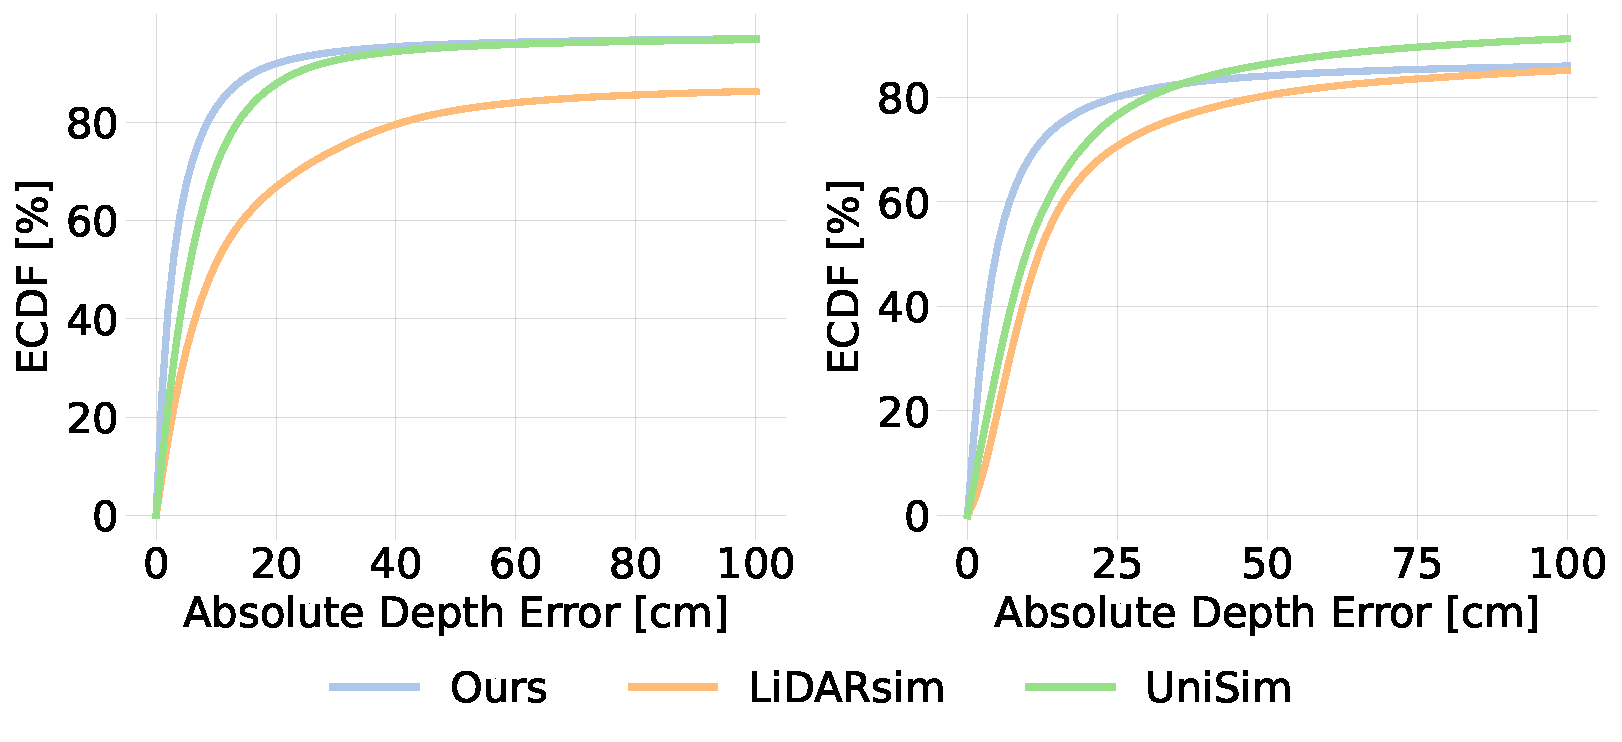
\includegraphics[width=1\columnwidth]{Figures/ecdf_3_methods.pdf}
   
        \caption{ECDF plots showcasing range errors across all the points (left) and specifically for points associated with dynamic vehicles (right). Our neural fields composition demonstrates superior performance over LiDARsim~\cite{manivasagam2020lidarsim} and UniSim~\cite{yang2023unisim}, especially in the context of dynamic vehicles.}
   \label{fig:ecdf}
   
\end{figure}
\begin{figure}[t]
    \centering
        \includegraphics[width=1\columnwidth]{Figures/errormap_static.pdf}
        
        \caption{Qualitative results of range estimation. Regions with gross errors (-100 \bwrDyNFL~100 cm) are highlighted.
        }
    \label{fig:error_map}
\end{figure}
\subsection{LiDAR novel view synthesis evaluation} \label{sec:lidar_eval}
\paragraph{LiDAR NVS in dynamic scenes.}

Quantitative comparisons with baseline methods are detailed in~\cref{tab:waymodynamic}. \dynfl notably outperforms LiDARsim~\cite{manivasagam2020lidarsim} and UniSim~\cite{yang2023unisim} in range reconstruction. This improvement is largely due to our SDF-based neural scene representation, which incorporates the physical aspects of LiDAR sensing. Additionally, our method employs a ray drop test when rendering multiple neural fields, leading to a more accurate reconstruction of dynamic vehicles, as evidenced in~\cref{fig:errormap_dynamic} and further supported by the data in~\cref{fig:ecdf}.



\paragraph{LiDAR NVS in static scenes.}
In addition to dynamic scenes, we evaluate \dynfl against baseline methods in static scenarios, with the results detailed in~\cref{tab:waymostatic} and~\cref{fig:error_map}. \dynfl excels in reconstructing geometry in most cases. A key observation is its superior performance in reconstructing planar regions (\eg the ground shown in~\cref{fig:error_map}), especially when compared to NFL~\cite{Huang2023nfl}, which also uses a neural field for surface representation. This improvement is largely due to the enhanced surface regularizations provided by our advanced SDF-based surface modeling approach.

 



\begin{table}[t]
    \setlength{\tabcolsep}{4pt}
    \renewcommand{\arraystretch}{1.2}
	\centering
	\resizebox{0.5\columnwidth}{!}{
    \small
    \begin{tabular}{l|ccc}
    \toprule
    Datasets  & MAE $\downarrow$ &  MedAE $\downarrow$ & CD $\downarrow$ \\
    \midrule
    TownClean~ & 26.7(\textcolor{green}{-1.5}) & 0.7(\textcolor{green}{-0.2}) & 6.7(\textcolor{green}{-0.5})\\
    Waymo Interp~ & 28.3 (\textcolor{red}{0.1}) & 4.7 (\textcolor{green}{-0.2}) & 12.5 (\textcolor{green}{-0.1})\\
    Waymo Dynamic~ & 30.8 (\textcolor{green}{-0.3}) & 3.0 (\textcolor{green}{-0.2}) & 10.9 (\textcolor{green}{-0.3})\\
    \bottomrule
    \end{tabular}
    }
    
	\caption{Ablation study of volume rendering for active sensing.}
	\label{tab:active_sensing}
\end{table}
\begin{table}[t]
    \setlength{\tabcolsep}{4pt}
    \renewcommand{\arraystretch}{1.2}
	\centering
	\resizebox{0.5\columnwidth}{!}{
    \small
    \begin{tabular}{l|ccc}
    \toprule
    Datasets  & MAE $\downarrow$ &  MedAE $\downarrow$ & CD $\downarrow$ \\
    \midrule
    TownReal~ & 33.9(\textcolor{green}{-3.3}) & 2.1(\textcolor{green}{-0.0}) & 10.4(\textcolor{green}{-1.2})\\
    Waymo Interp~ & 28.3 (\textcolor{green}{-0.3}) & 4.7 (\textcolor{green}{-0.1}) & 12.5 (\textcolor{green}{-0.3})\\
    \bottomrule
    \end{tabular}
    }
    
	\caption{Ablation study of the surface points' SDF regularisation.}
	\label{tab:surface_sdf}
\end{table}
\begin{figure}[t]
  \centering
   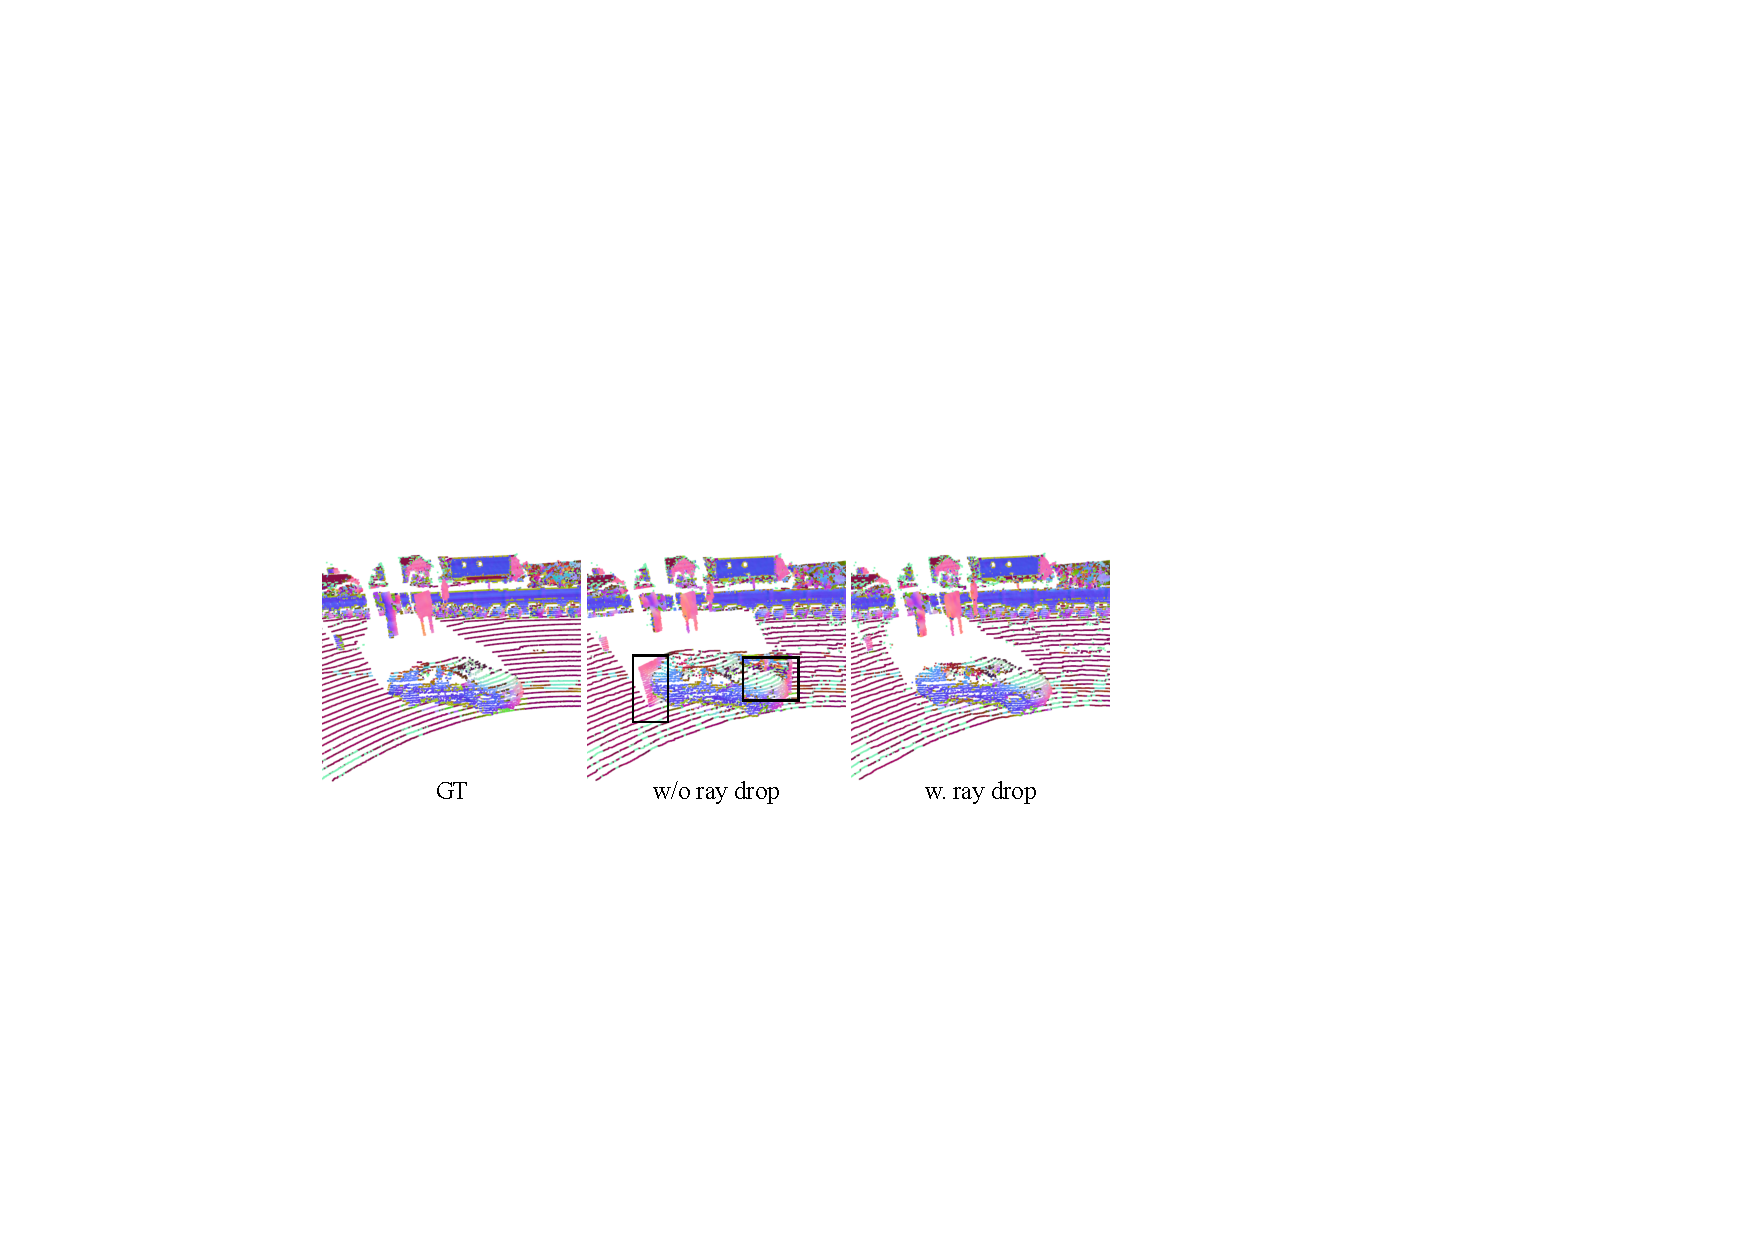
\includegraphics[width=1\linewidth]{Figures/intersectiontest.pdf}
   
   \caption{
   Qualitative results on \textit{Waymo Dynamic} dataset. Our model equipped with a ray drop module effectively composites multiple neural fields, re-simulating LiDAR scans of high quality.
   }
   % \caption{These figures exemplify the effectiveness of our field composition method leveraging ray drop probability from dynamic neural field. When all intersected rays are rendered for the dynamic neural field, noticeable artifacts appear due to disturbances from irrelevant fields (middle figure). The figures on the right showcase the complete composition method.
   % }
   % \caption{
   % }
    
   \label{fig:ablation_raydrop}
\end{figure}

\begin{figure}[t]
    \centering
        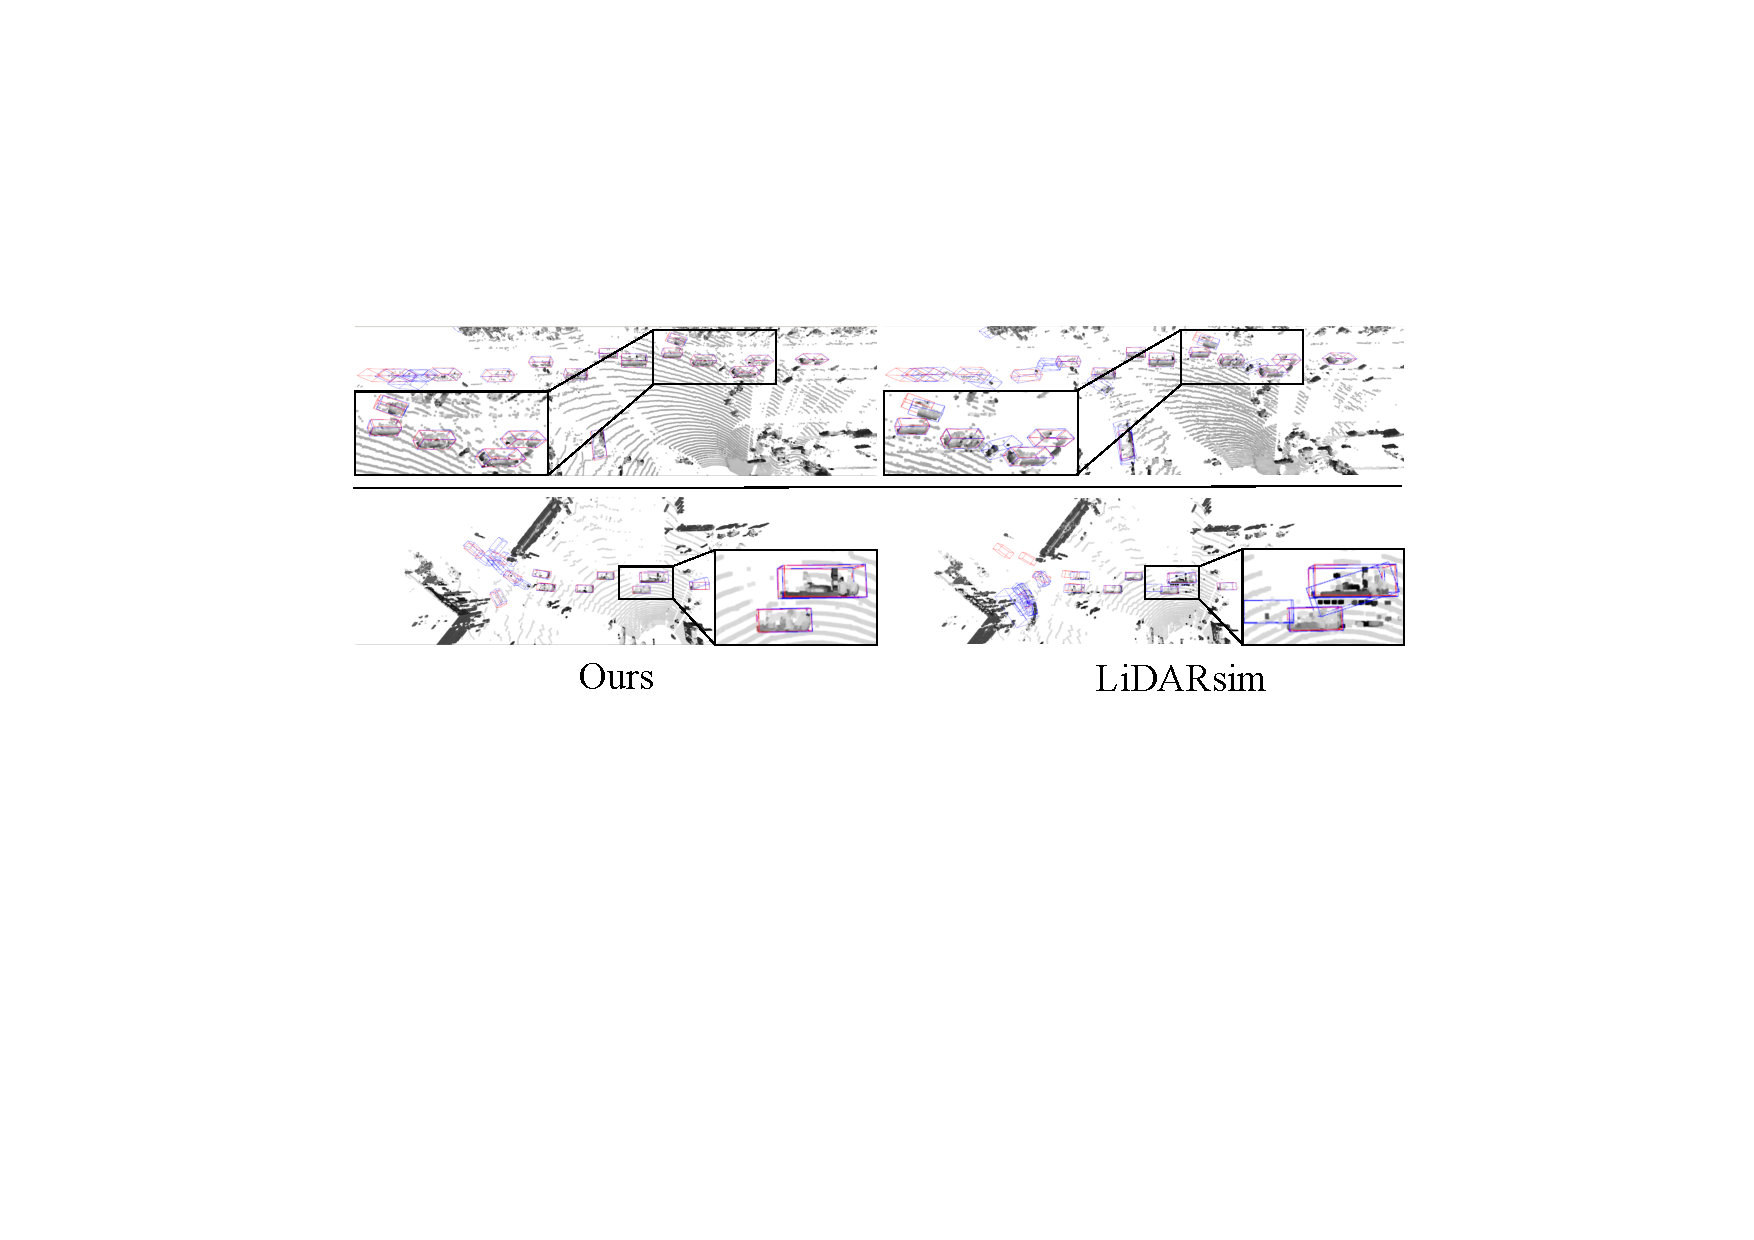
\includegraphics[width=0.8\columnwidth]{Figures/detection_result.pdf}
        \caption{Object detection results on \textit{Waymo Dynamic} dataset. The ground truth and predicted bounding boxes are marked in \textcolor{red}{red} and \textcolor{blue}{blue}, respectively.}
    \label{fig:detection}
    
\end{figure}
\begin{figure*}[t]
    \centering
        \includegraphics[width=1.0\textwidth]
        {Figures/sensor_manipulation.pdf}
        
        \caption{LiDAR novel view synthesis by changing sensor elevation angle~($\theta$), poses~($x,y,z$) and number of beams on \textit{Waymo Dynamic} dataset. The points are color-coded by the intensity values (0 \bwrDyNFL~0.25).}
    \label{fig:lidar_nvs}
\end{figure*}
% \begin{table}[t]
% 	\centering
% 	\resizebox{0.8\columnwidth}{!}{
% 		\begin{tabular}{@{}lcccccccc@{}}
% 			\toprule
%              & \multicolumn{1}{c}{GT} & \multicolumn{3}{c}{Ours} & \multicolumn{3}{c}{LiDARSim\cite{manivasagam2020lidarsim}} \\
% 			  \cmidrule(r){2-2}\cmidrule(r){3-5} \cmidrule(l){6-8}
% 			Threshold & AP$\uparrow$ & \multicolumn{1}{c}{AP$\uparrow$}& \multicolumn{1}{c}{Agg.$\uparrow$}& \multicolumn{1}{c}{Dyn. Agg.$\uparrow$} & \multicolumn{1}{c}{AP$\uparrow$} & \multicolumn{1}{c}{Agg.$\uparrow$}& \multicolumn{1}{c}{Dyn. Agg.$\uparrow$} \\
% 			\midrule
% 			IoU$>$0.7 &0.85  &0.86 & \textbf{0.77}& \textbf{0.71}& \textbf{0.90} & 0.76 & 0.68\\
% 			IoU$>$0.5 &\textbf{0.98}  & 0.96 & \textbf{0.87}& \textbf{0.76}& 0.95 & 0.86& \textbf{0.76} \\
% 			\bottomrule
% 		\end{tabular}
% 	}
% 	\caption{Object detection results on \textit{Waymo Dyanmic} datasets.}
    
% 	\label{tab:detection}
% \end{table}

\begin{table}[t]
	\centering
		\begin{tabularx}{\columnwidth}{l|YYYYYYY}
			\toprule
             & \multicolumn{1}{c}{GT} & \multicolumn{3}{c}{Ours} & \multicolumn{3}{c}{LiDARSim\cite{manivasagam2020lidarsim}} \\
			  \cmidrule(r){2-2}\cmidrule(r){3-5} \cmidrule(l){6-8}
			Threshold & AP$\uparrow$ & \multicolumn{1}{c}{AP$\uparrow$}& \multicolumn{1}{c}{Agg.$\uparrow$}& \multicolumn{1}{c}{Dyn. Agg.$\uparrow$} & \multicolumn{1}{c}{AP$\uparrow$} & \multicolumn{1}{c}{Agg.$\uparrow$}& \multicolumn{1}{c}{Dyn. Agg.$\uparrow$} \\
			\midrule
			IoU$>$0.7 &0.85  &0.86 & \textbf{0.77}& \textbf{0.71}& \textbf{0.90} & 0.76 & 0.68\\
			IoU$>$0.5 &\textbf{0.98}  & 0.96 & \textbf{0.87}& \textbf{0.76}& 0.95 & 0.86& \textbf{0.76} \\
			\bottomrule
		\end{tabularx}
	\caption{Object detection results on \textit{Waymo Dyanmic} datasets.}
    
	\label{tab:detection}
\end{table}
% \begin{table}[t]
% \setlength{\tabcolsep}{4pt}
% \renewcommand{\arraystretch}{1.2}
% \centering
% \resizebox{0.8\columnwidth}{!}{
% \begin{tabular}{l|ccc|ccc}
% \toprule
% & \multicolumn{3}{c|}{Vehicle} & \multicolumn{3}{c}{Background} \\
% Method & Recall $\uparrow$ & Precision $\uparrow$ & IoU $\uparrow$ & Recall $\uparrow$ & Precision $\uparrow$ & IoU $\uparrow$ \\
% \midrule
% i-NGP~\cite{muller2022instant} & \underline{93.2} & 85.9 & 80.9 & 98.3 & \underline{99.2} & 97.6\\
% DS-NeRF~\cite{deng2021depth} & 90.7 & \underline{87.1} & 80.2 & \underline{98.5} & 98.9 & 97.4\\
% URF~\cite{rematas2021urban} & 87.8 & 81.7 & 73.7 & 98.0 & 98.4 & 96.5\\
% Lidarsim~\cite{manivasagam2020lidarsim} & 90.5 & 70.5 & 65.9 & 94.9 & 99.0 & 94.0\\
% NFL density~\cite{Huang2023nfl}& \textbf{95.9} & 87.0 & \textbf{83.9} & 98.3 & \textbf{99.5} & \textbf{97.8}\\
% Ours & 90.5 & \textbf{89.2} & \underline{82.3} & \textbf{98.8} & 98.9 & \underline{97.7}\\
% \bottomrule
% \end{tabular}
% }
% 
% \caption{Semantic segmentation results on \textit{Waymo NVS} dataset.}
% \label{tab:sem_seg_nvs}
% \end{table}



\begin{table}[t]
\setlength{\tabcolsep}{4pt}
\renewcommand{\arraystretch}{1.2}
\centering
\resizebox{0.99\columnwidth}{!}{
\begin{tabular}{l|ccc|ccc}
\toprule
& \multicolumn{3}{c|}{Vehicle} & \multicolumn{3}{c}{Background} \\
Method & Recall $\uparrow$ & Precision $\uparrow$ & IoU $\uparrow$ & Recall $\uparrow$ & Precision $\uparrow$ & IoU $\uparrow$ \\
\midrule
i-NGP~\cite{mueller2022instant} & 91.8 & 83.6 & 78.1 & 97.9 & 99.2 & 97.1\\
DS-NeRF~\cite{kangle2021dsnerf} & 89.3 & 84.8 & 77.3 & 98.1 & 98.8 & 97.0\\
URF~\cite{rematas2021urban} & 86.9 & 79.8 & 72.0 & 97.7 & 98.5 & 96.2\\
Lidarsim~\cite{manivasagam2020lidarsim} & 89.6 & 68.9 & 64.0 & 94.5 & 98.9 & 93.5\\
NFL~\cite{Huang2023nfl}& \textbf{94.5} & 84.8 & 80.9 & 97.8 & \textbf{99.4} & \textbf{97.3}\\
Ours & 90.5 & \textbf{88.4} & \textbf{81.1} & \textbf{98.5} & 98.7 & \textbf{97.3}\\
\bottomrule
\end{tabular}
}

\caption{Semantic segmentation results on \textit{Waymo NVS} dataset.}
\label{tab:sem_seg_nvs_ours}

\end{table}
\begin{figure}[t]
    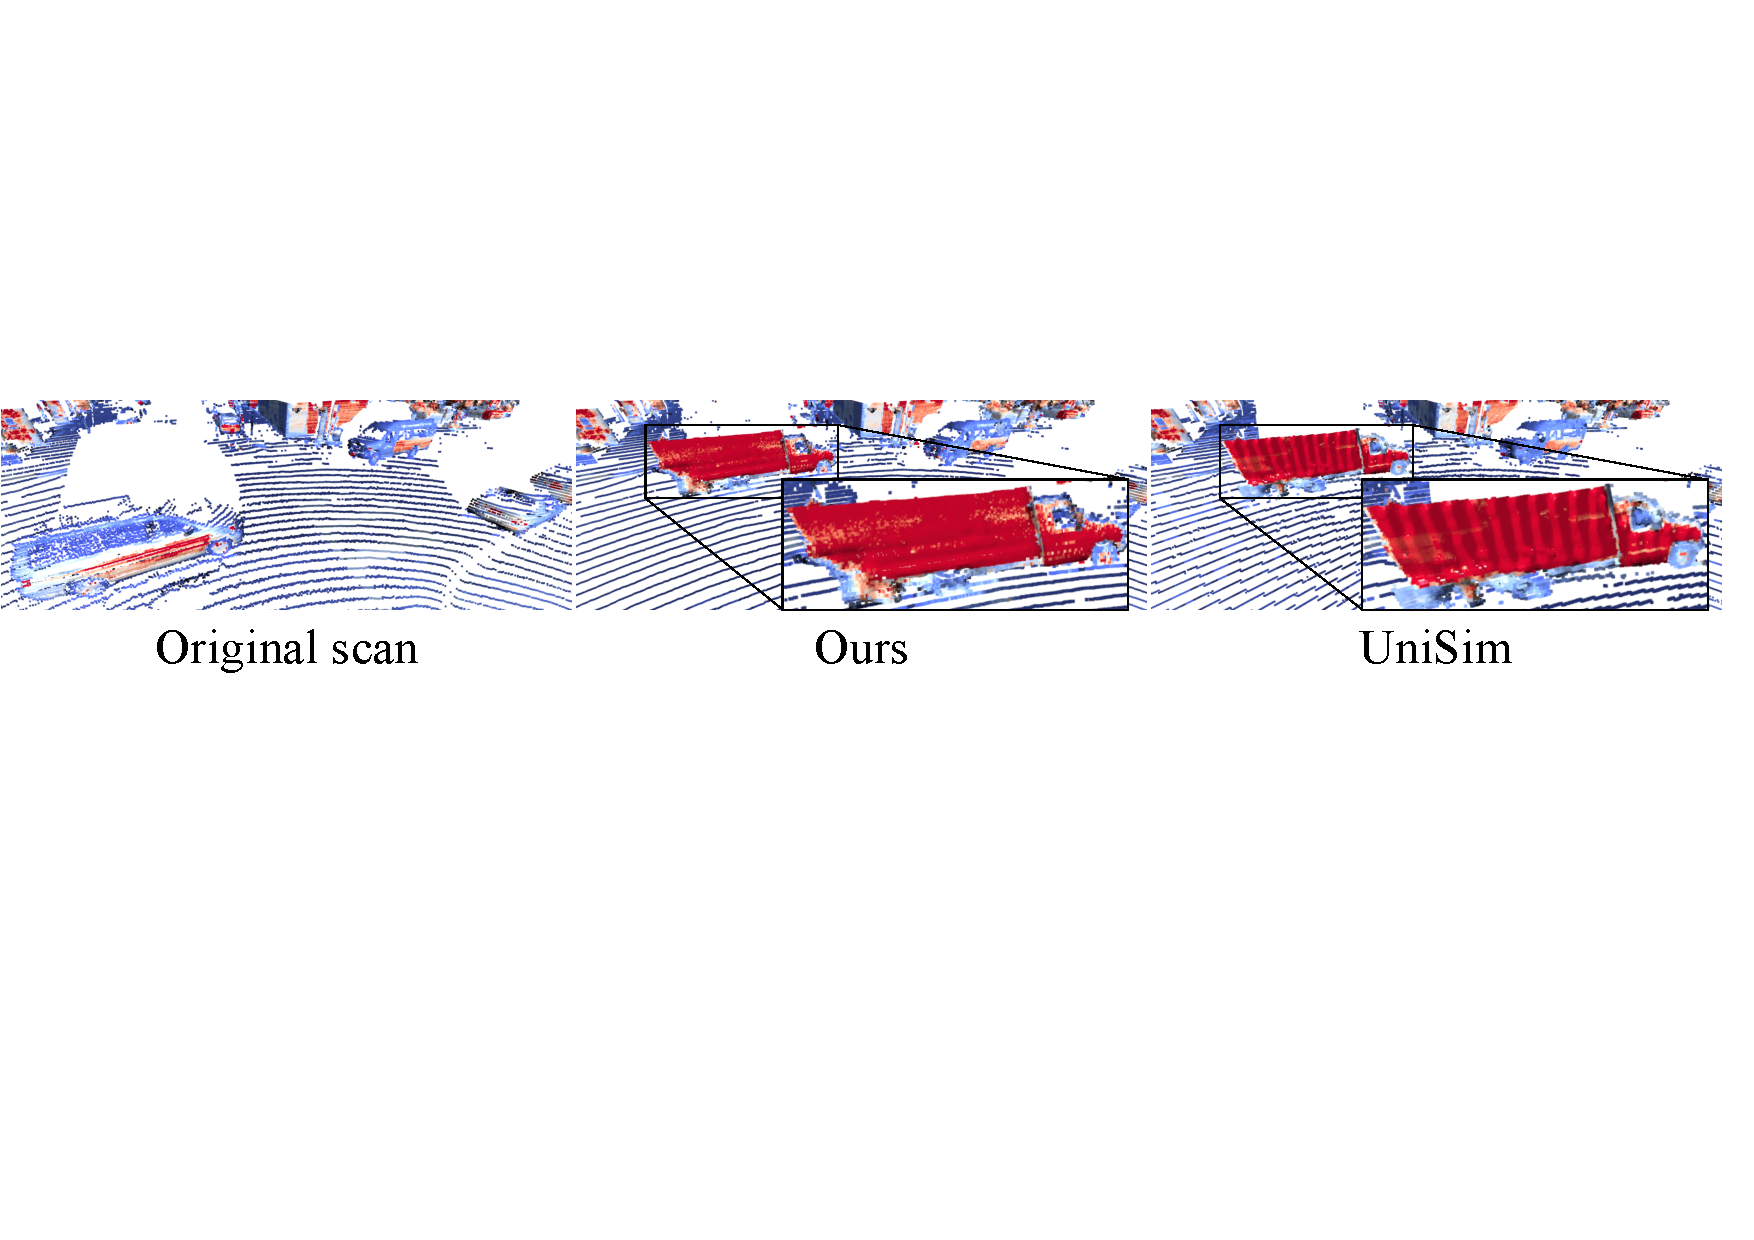
\includegraphics[width=1.0\linewidth]{Figures/vehicle_insertion.pdf}
    
    \caption{
    Qualitative results of object removal and insertion. \dynfl seamlessly inserts the neural asset (truck) into a new scene attributed to our superior compositional rendering scheme. In contrast, UniSim~\cite{yang2023unisim} struggles to accurately model geometry.
    }
    \label{fig:vehicle_insertion}
\end{figure}
\begin{figure}[t]
    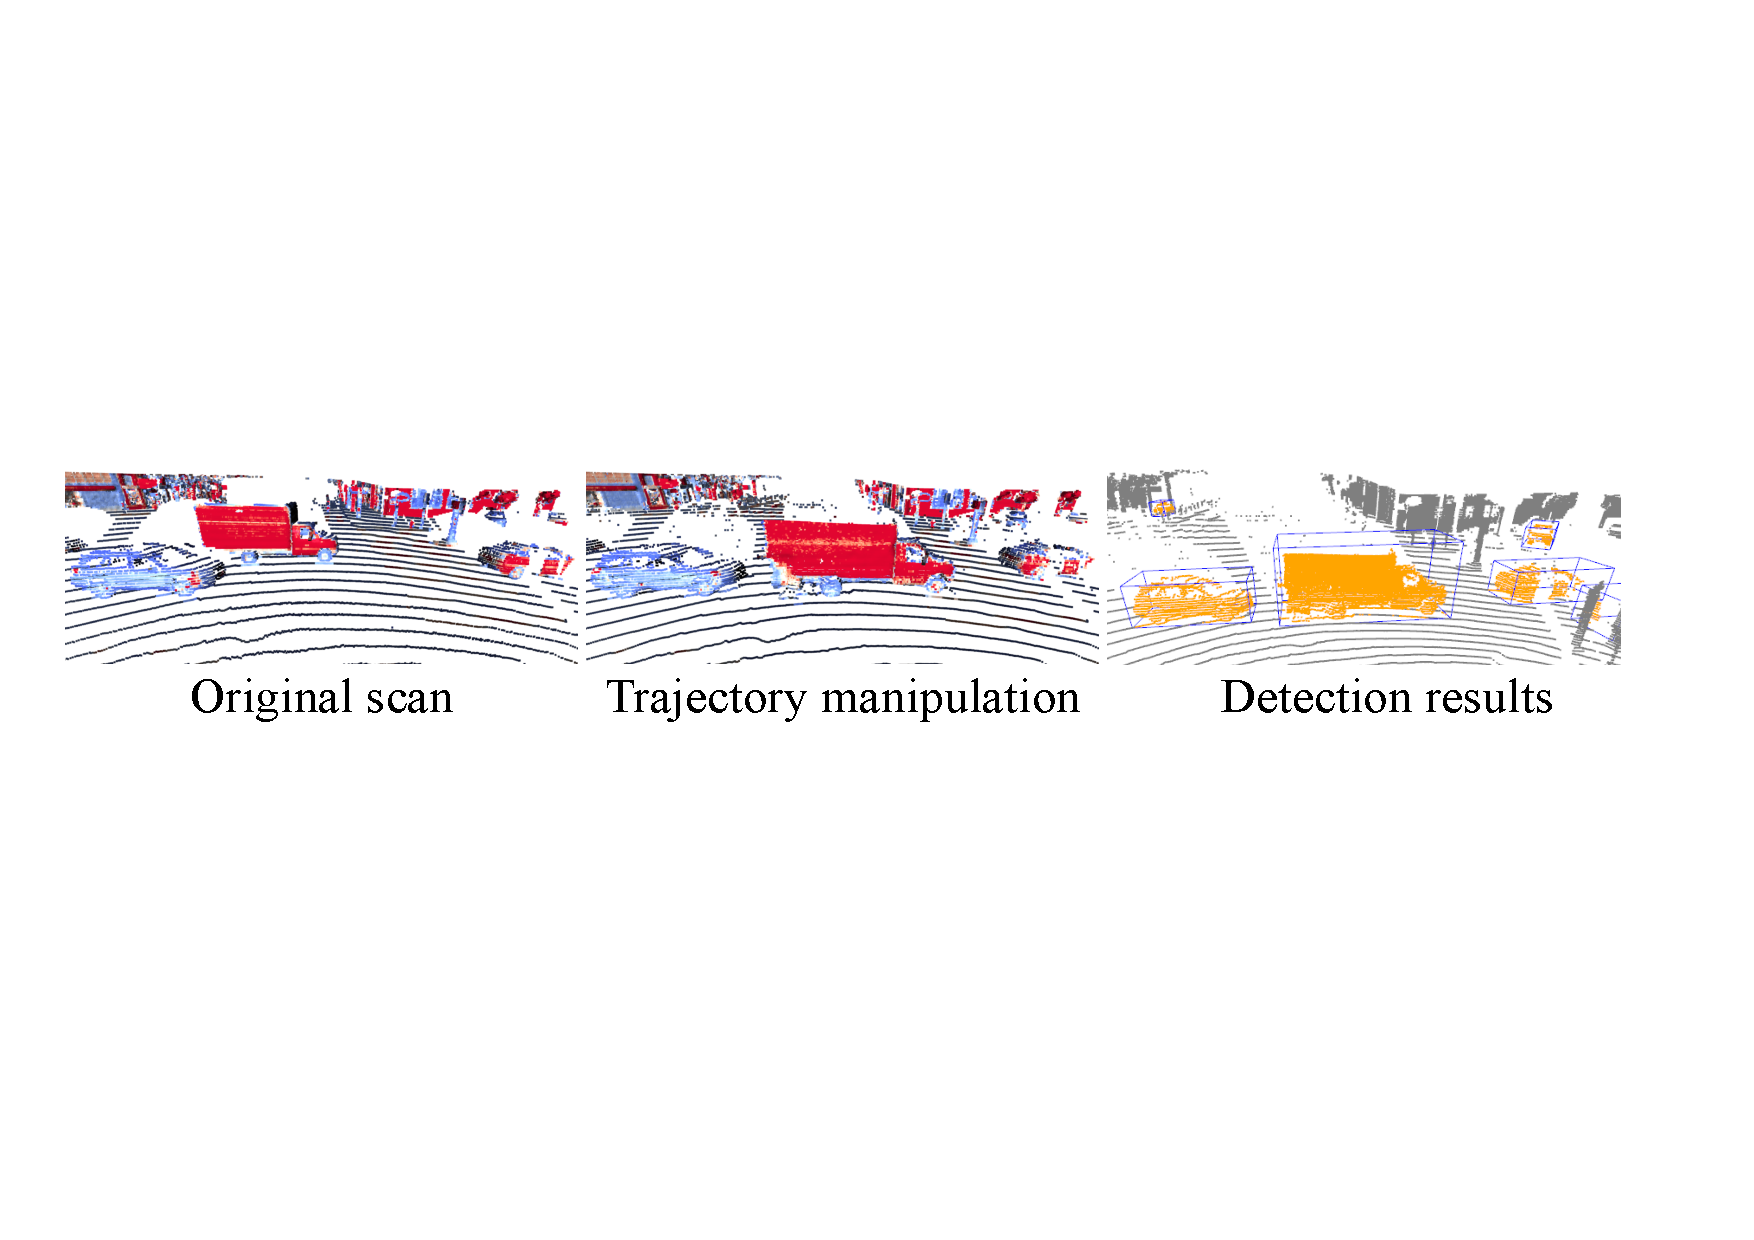
\includegraphics[width=1.0\columnwidth]{Figures/trajectory_manipulation.pdf}
    
    \caption{Qualitative results of object trajectory manipulation. The truck can be successfully detected after manipulation, indicating high-realism LiDAR re-simulation achieved by \dynfl.}
    \label{fig:traj}
    
\end{figure}


\subsection{Ablation study}
\paragraph{SDF-based volume rendering for active sensing.}
We begin by assessing the efficacy of our SDF-based volume rendering for active sensor, the results are shown in~\cref{tab:active_sensing}. When compared to our baseline that uses the SDF-based volume rendering for passive sensing, \dynfl demonstrates enhanced performance in both synthetic (\textit{TownClean}) and real-world (\textit{Waymo Interp} and \textit{Waymo Dynamic}) datasets, indicating the importance of incorporating the physical sensing process of LiDAR in addressing the inverse problem.


\paragraph{Neural fields composition.} 
To validate the efficacy of our two-stage neural field composition approach, we compare it with an alternative approach utilized in UniSim~\cite{yang2023unisim}. The results are shown in~\cref{tab:waymodynamic}. UniSim~\cite{yang2023unisim} blends different neural fields by sampling points from all intersected neural fields, followed by a single evaluation of volume rendering to produce the final LiDAR scan. In contrast, our method independently renders from each intersecting neural field first, and then combines these measurements into a final measurement using a ray drop test (\cf~\cref{fig:ablation_raydrop}). This approach leads to a notable improvement in geometry reconstruction over UniSim~\cite{yang2023unisim}, exemplified by our method halving the Median Absolute Error (MedAE) across all points. This enhancement is even more evident when focusing solely on points related to dynamic vehicles (\cf~\cref{fig:ecdf}).
% 

\paragraph{Surface points' SDF constraint.}
We examine the importance of the surface points' SDF constraint discussed in ~\cref{sec:optmisation} on \textit{Town Real} and \textit{Waymo Interp} datasets. The results shown in \cref{tab:surface_sdf} suggest that our method yields improved geometry reconstruction quality by additionally enforcing LiDAR points to have zero SDF values. 


\subsection{Auxiliary task evaluations} 
\label{sec:downstream}
To assess the fidelity of our neural re-simulation and gauge the domain gap between re-simulated and real scans, we evaluate their applicability in two downstream tasks: object detection and semantic segmentation.


\paragraph{Object detection.}
We utilize the pre-trained FSDv2~\cite{fan2023fsdv2} model for object detection and conduct evaluations on the re-simulated LiDAR scans within the \textit{Waymo Dynamic} dataset. Our results are compared against those from LiDARsim~\cite{manivasagam2020lidarsim}, with the findings detailed in~\cref{tab:detection} and~\cref{fig:detection}. Notably, \dynfl exhibits a more substantial detection agreement with the predictions on real LiDAR scans. This indicates a higher fidelity in our re-simulations and a reduced domain gap relative to actual scans.




\paragraph{Semantic segmentation.}
For semantic segmentation, we use the pre-trained SPVNAS model~\cite{tang2020searching}, with the results presented in~\cref{tab:sem_seg_nvs_ours}. \dynfl improves over baseline methods according to most evaluation metrics, underscoring the realism of our re-simulated LiDAR scans.



\subsection{Scene editing}
Beyond LiDAR novel view synthesis by adjusting the sensor configurations (\cf \cref{fig:lidar_nvs}), we additionally demonstrate the practicality of our compositional neural fields approach through two scene editing applications.


\paragraph{Insert object from one scene into another.}
Our explicit neural scene de-composition and flexible composition technique enable seamless insertion and removal of neural assets across scenes. As demonstrated in~\cref{fig:vehicle_insertion}, we are able to replace a car from one scene with a truck from another scene, achieving accurate reconstruction of both geometry and intensity. In contrast, UniSim~\cite{yang2023unisim} struggles to preserve high quality geometry. This highlights the significant potential of our approach in generating diverse and realistic LiDAR scans for autonomous driving scenarios.


\paragraph{Manipulate the trajectory of dynamic objects.}
\dynfl also facilitates the manipulation of moving objects' trajectories by simply adjusting their relative poses to the canonical bounding box. Representative results are shown in ~\cref{fig:traj}. The high realism of our re-simulation is also indicated by the successful detection of inserted virtual objects.
